\documentclass{jsarticle}
\usepackage[dvipdfmx]{graphicx}
\usepackage{amsmath}
\usepackage{amssymb}
\usepackage{bm}
\usepackage{here}
\usepackage{mathtools}

\DeclareMathOperator*{\argmin}{argmin}
\DeclareMathOperator*{\argmax}{argmax}

\title{ART.T458 Advanced Machine Learning Midterm Assignment}

\author{21M30821 山上理久}

\begin{document}
\maketitle

\section*{Problem 1 (10pts)*}
線形ロジスティック回帰による二値分類を考える。$x \in \mathbb R^d$をd次元の入力ベクトル、$w \in \mathbb R^d$をモデルのパラメータとする。
分類器は,$f(x) = 2 [\![w^\top x]\!] > 0 - 1$で表され,$c$は,$c$が真であれば1を,そうでなければ0を返す指示関数を表す。
教師付きデータセット${\bm x_i, y_i}^n_{i=1}$を用いて,ロジスティック回帰の最適化問題を考える.この最適化問題は次のように書くことができる。
\begin{align*}
  \hat{\bm w} &=  \argmin_{\bm w} J(\bm w) \\
  J(\bm w) &:= \sum_{i=1}^n (\ln (1+\exp(-y_i\bm w^\top \bm x_i))) + \lambda\bm w^\top\bm w.
\end{align*}
人工的なデータセット(Toy Dataset IVを使用)を用いて、以下のようにの最適化手法を実装することを考える。

\begin{enumerate}
  \item バッチ式最急降下法の導入
  
  バッチ式最急降下法を実装し、二値分類を行った結果は図1、誤分類は図2である。以下、誤分類を表す図では赤が正常な分類、青が誤分類を意味する。
  \begin{figure}[htbp]
    \centering
    \begin{minipage}{0.4\linewidth}
      \centering
      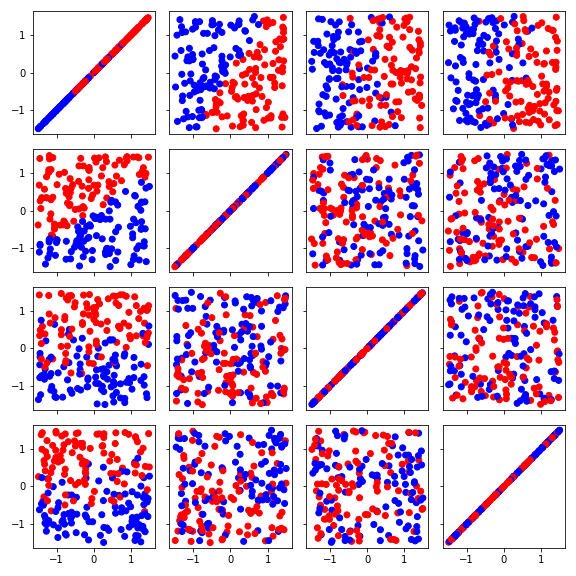
\includegraphics[width=.9\textwidth]{image/1-1-1.png}
    \caption{バッチ式最急降下法の二値分類の結果}
    \end{minipage}
    \begin{minipage}{0.4\linewidth}
      \centering
      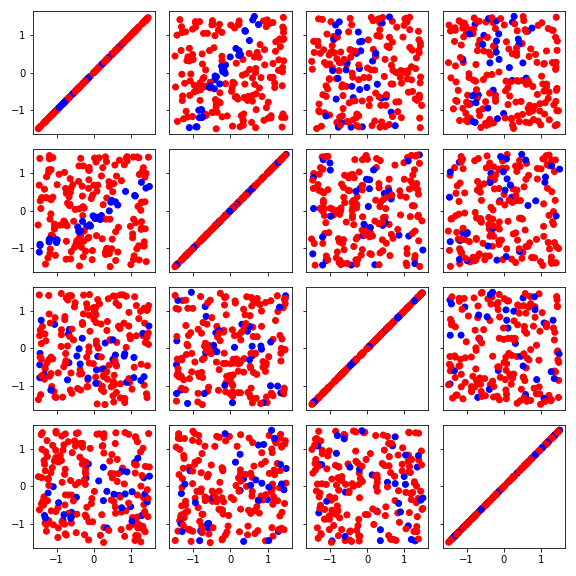
\includegraphics[width=.9\textwidth]{image/1-1-2.png}
    \caption{バッチ式最急降下法の二値分類の誤分類}
    \end{minipage}
  \end{figure}

  \item ニュートン法の導入
  
  ニュートン法を実装し、二値分類を行った結果は図3、誤分類は図4である。
  \begin{figure}[htbp]
    \centering
    \begin{minipage}{.4\linewidth}
      \centering
      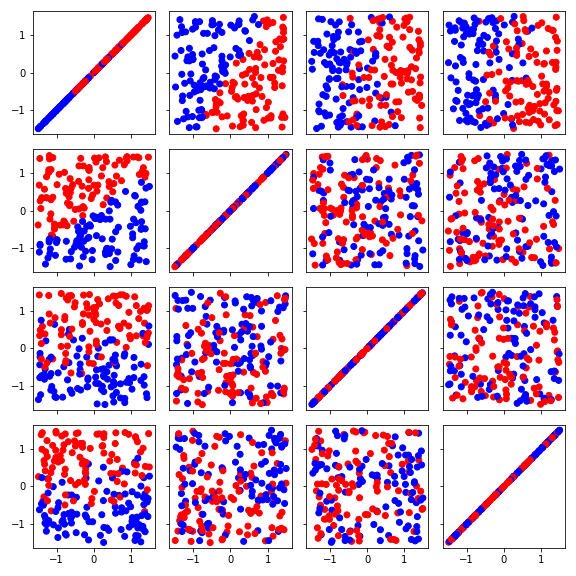
\includegraphics[width=.9\textwidth]{image/1-2-1.png}
      \caption{ニュートン法の二値分類の結果}
    \end{minipage}
    \begin{minipage}{.4\linewidth}
      \centering
      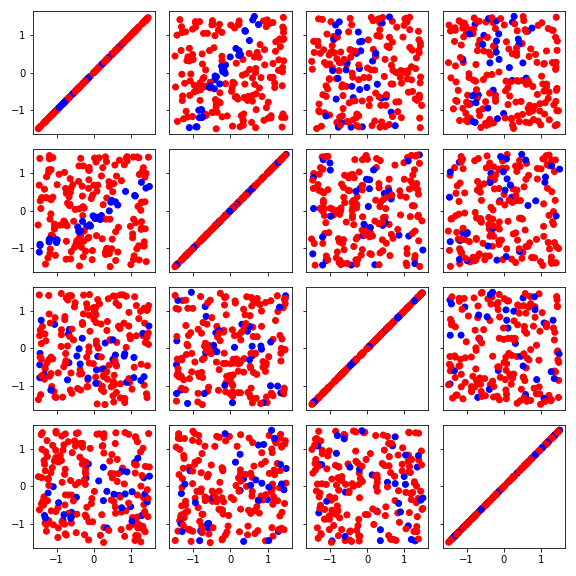
\includegraphics[width=.9\textwidth]{image/1-2-2.png}
      \caption{ニュートン法の二値分類の誤分類}
    \end{minipage}
  \end{figure}
  
  \item 上記2つの最適化手法の性能を比較するために、$|J(\bm w^{(t)}) - J(\hat{\bm w})|$ を片対数プロットで図示する。
  
  \begin{figure}[htbp]
    \centering
    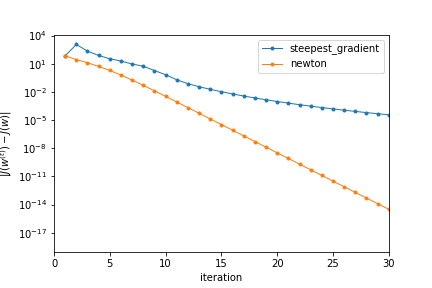
\includegraphics[width=.7\textwidth]{image/1-3.png}
    \caption{2つの最適化手法の性能の比較}
  \end{figure}

  \item マルチクラス版ロジスティック回帰(Toy Dataset Vを使用)にニュートン法と単純な最勾配法を導入し、上記の二値ロジスティック回帰と同じ実験を行う。
  
  バッチ式最急降下法を実装し、マルチクラス分類を行った結果と誤分類は下図の通りである。
  \begin{figure}[htbp]
    \centering
    \begin{minipage}{0.4\linewidth}
      \centering
      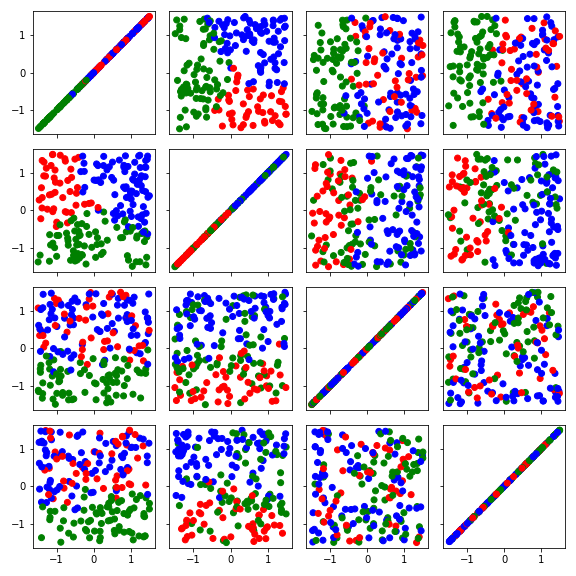
\includegraphics[width=.9\textwidth]{image/1-4-1.png}
    \caption{バッチ式最急降下法のマルチクラス分類の結果}
    \end{minipage}
    \begin{minipage}{0.4\linewidth}
      \centering
      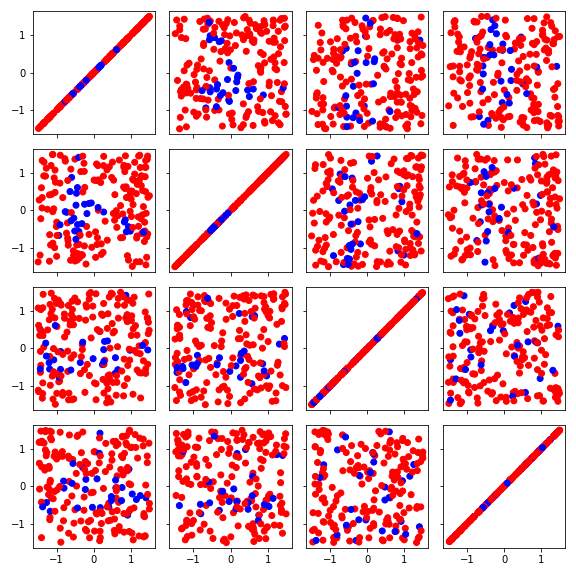
\includegraphics[width=.9\textwidth]{image/1-4-2.png}
    \caption{バッチ式最急降下法のマルチクラス分類の誤分類}
    \end{minipage}
  \end{figure}

  ニュートン法を実装し、マルチクラス分類を行った結果と誤分類は下図の通りである。
  \begin{figure}[htbp]
    \centering
    \begin{minipage}{0.4\linewidth}
      \centering
      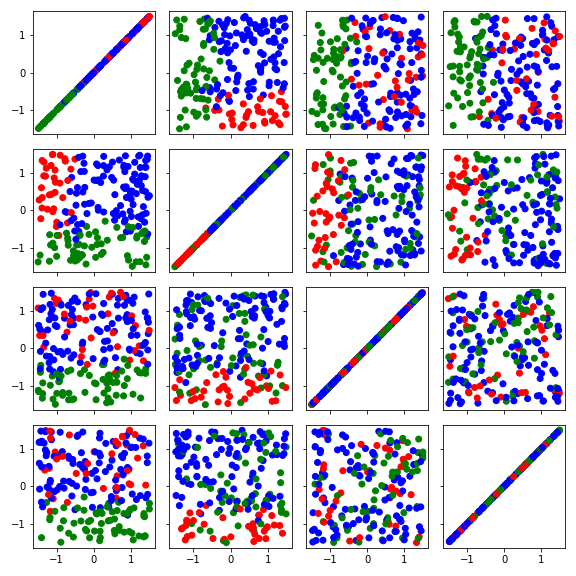
\includegraphics[width=.9\textwidth]{image/1-4-3.png}
    \caption{ニュートン法のマルチクラス分類の結果}
    \end{minipage}
    \begin{minipage}{0.4\linewidth}
      \centering
      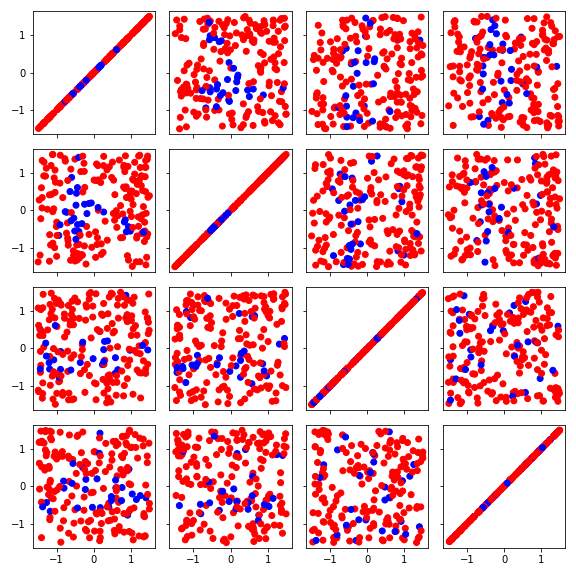
\includegraphics[width=.9\textwidth]{image/1-4-4.png}
    \caption{ニュートン法のマルチクラス分類の誤分類}
    \end{minipage}
  \end{figure}
  
\end{enumerate}

\section*{Problem 2 (5 pts)*}
線形回帰に平方損失とL1正則化を採用したlassoを考える。この問題では、近似勾配法(PG)を採用する。議論を簡単にするために、以下の目的を使用する。
\begin{align*}
  \hat{\bm w} = \argmin_{w} \left((\bm w-\bm\mu)\top \bm A(\bm w-\bm\mu)+\lambda||\bm w||_1\right).
\end{align*}
lassoのPGを実装し、いくつかの条件で結果を示す。
この問題では、同じ学習率$\eta_t = L_{-1}$を使用する。ここで、$L$は目的の勾配のリプシッツ定数を表し、ヘシアン行列$2\bm A$から導かれる(つまり、学習率の逆数として$2\bm A$の最大固有値を使用する:$\eta_t^{-1}-1$)。
\begin{enumerate}
  \item PGの結果を、繰り返し回数に応じて$||\bm w^{(t)} − \hat{\bm w}||$を片対数プロットで示す。次の条件を使用します。
  $$
  A=\begin{pmatrix}
  3& 0.5 \\
  0.5& 1
  \end{pmatrix}, \mu^\top=(1 2).
  $$
  L1正則化の特性を確認するために、$\lambda = 2, 4, 6$で実験を行う。
  $\lambda = 2, 4, 6$で実験を行った結果は下図の通りである。
  \begin{figure}[htbp]
    \centering
    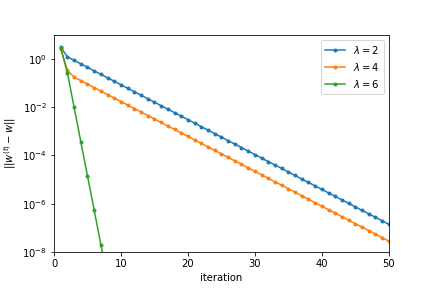
\includegraphics[width=.7\linewidth]{image/2.png}
    \caption{$\lambda$の違いによるL1正則化の特性の違い}
  \end{figure}
\end{enumerate}


\section*{Problem 3 (15 pts)*}
サポート・ベクトル・マシンの双対(L2正則化されたヒンジ・ロスに基づくバイナリ分類器)を考える。この分類の元々の最適化問題は,次のように表される。
\begin{align*}
  \hat{\bm w} = \argmin_{\bm w\in \mathbb R^d}\left(\sum_{i=1}^n\max(0, 1 − y_i\bm w^\top \bm x_i) + \lambda||\bm w||_2^2\right),
\end{align*}
ここで $\bm x_i \in \mathbb R^d$, $\bm w \in \mathbb R^d$, $y_i \in {±1}$, $\lambda > 0$はそれぞれ$i$番目の入力変数、パラメータベクトル、$i$番目の入力データのラベル、正則化項の係数を表す。
\begin{enumerate}
  \item この最適化の双対ラグランジュ関数が次のように書けることを検証する。
  \begin{align*}
    \nonumber
    \mathrm{maximize}_{ \bm\alpha\in\mathbb R^n}&\quad − \frac{1}{4\lambda} \bm\alpha^\top\bm K\bm\alpha + \bm\alpha^\top\bm 1,  \\
    \mathrm{subject\ to}&\quad \bm 0\le\bm\alpha\le\bm 1
  \end{align*}
  ここで、$\bm 1$, $\bm 0$は、それぞれ$1$, $0$を要素とするn次元のベクトルを表し、$K \in \mathbb R^{n×n}$は対称正方行列を表し、その$i$番目の行と$j$番目の列の要素は$y_iy_j\bm x_i^\top\bm x_j$である。

  主問題を$\bm\xi$を用いて再定義する。
  \begin{align*}
    \mathrm{maximize}_{\bm w,\bm\xi}&\quad \xi^\top\bm 1 + \lambda\bm w^\top\bm w \\
    \mathrm{subject\ to}&\quad \xi_i\ge1-y_i\bm w^\top\bm x_i \quad i=1,\cdots,n\\
    &\quad \bm\xi\ge\bm0
  \end{align*}
  ラグランジェ乗数$\bm\alpha,\bm\beta(\ge\bm0)$を用いて, 以下のラグランジェ関数を考える。
  \begin{align*}
    L(\bm w,\bm\xi,\bm\alpha,\bm\beta) = \bm\xi^\top\bm 1 + \lambda\bm w^\top\bm w + \sum_{i=1}^n \alpha_i\left(1-y_i\bm w^\top\bm x_i - \xi_i\right) + \sum_{j=1}^n-\beta_j\xi_j
  \end{align*}
  このとき、
  \begin{align*}
    \begin{dcases}
      \frac{\partial L}{\partial \bm w} = 2\lambda\bm w - \sum_{i=1}^n\alpha_iy_i\bm x_i\\
      \frac{\partial L}{\partial \bm\xi} = \bm1-\bm\alpha-\bm\beta
    \end{dcases}
  \end{align*}
  $\left.\frac{\partial L}{\partial \bm w}\right|_{(\bm w,\bm\xi,\bm\alpha,\bm\beta)=(\hat{\bm w},\hat{\bm\xi},\hat{\bm\alpha},\hat{\bm\beta})} = \left.\frac{\partial L}{\partial \bm\xi}\right|_{(\bm w,\bm\xi,\bm\alpha,\bm\beta)=(\hat{\bm w},\hat{\bm\xi},\hat{\bm\alpha},\hat{\bm\beta})}=\bm0$より、
  \begin{align}
    \begin{dcases}
      \hat{\bm w} = \frac{1}{2\lambda}\sum_{i=1}^n\hat{\alpha_i}y_i\bm x_i \\
      \hat{\bm\alpha}+\hat{\bm\beta}=\bm1
    \end{dcases}
  \end{align}
  よって、
  \begin{align*}
    L(\hat{\bm w},\hat{\bm\xi},\hat{\bm\alpha},\hat{\bm\beta}) &= \hat{\bm\xi}^\top\bm 1 + \lambda\hat{\bm w}^\top\hat{\bm w} + \sum_{i=1}^n \hat{\alpha_i}\left(1-y_i\hat{\bm w}^\top\bm x_i - \hat{\xi_i}\right) + \sum_{j=1}^n-\hat\beta_j\hat\xi_j \\
    &= \hat{\bm\xi}^\top(\bm 1 -\hat{\bm\alpha}-\hat{\bm\beta})+ \lambda||\frac{1}{2\lambda}\sum_{i=1}^n\hat{\alpha_i}y_i\bm x_i||_2^2 
    + \sum_{i=1}^n \hat\alpha_i
    - \sum_{i=1}^n \hat\alpha_iy_i\left(\frac{1}{2\lambda}\sum_{j=1}^n\hat{\alpha_j}y_j\bm x_j^\top\right)\bm x_i \\
    &= \lambda||\frac{1}{2\lambda}\sum_{i=1}^n\hat{\alpha_i}y_i\bm x_i||_2^2 
    + \sum_{i=1}^n \hat\alpha_i
    - \sum_{i=1}^n \hat\alpha_iy_i\left(\frac{1}{2\lambda}\sum_{j=1}^n\hat{\alpha_j}y_j\bm x_j^\top\right)\bm x_i \\
    &= -\frac{1}{2\lambda}\sum_{i=1}^n\sum_{j=1}^n\hat{\bm\alpha_i}\hat{\bm\alpha_j}y_iy_j\bm x_i^\top\bm + \hat{\bm\alpha}^\top\bm1 \\
    &= -\frac{1}{2\lambda}\hat{\bm\alpha}^\top\bm K\hat{\bm\alpha}+\hat{\bm\alpha}^\top\bm1\quad\left(\{\bm K\}_{i,j}=y_iy_j\bm x_i^\top\bm x_j\right)
  \end{align*}
  以上より、$\hat{\bm\alpha},\hat{\bm\beta}$を$\bm\alpha,\bm\beta$とすることによって、
  \begin{align*}
    \mathrm{maximize}_{\bm \alpha\in\mathbb{R}^n}&\quad -\frac{1}{2\lambda}\bm\alpha^\top\bm K\bm\alpha \\
    \mathrm{subject\ to}&\quad \bm0\le\bm\alpha\le\bm1\quad(\because \bm\alpha = \bm1-\bm\beta\le\bm1)
  \end{align*}
  が導出される。

  \item KKT条件から、$\alpha$で与えられる最適な重みパラメータ$\bm w$が次のように書けることを検証する。
  \begin{align*}
    \hat{\bm w} = \frac{1}{2\lambda}\sum_{i=1}^n \alpha_iy_i\bm x_i
  \end{align*}
  式(1)より、
  \begin{align*}
    \hat{\bm w} = \frac{1}{2\lambda}\sum_{i=1}^n \alpha_iy_i\bm x_i
  \end{align*}
  が導出される。

  \item 負の双対ラグランジュ関数の最小化を、投影勾配を用いて実施する。妥当性については、双対ラグランジュ関数のスコアと、ヒンジ損失関数と正則化の和を、それぞれ反復回数に対して示す。双対性ギャップが0になると収束することを確認する。ここでは、投影勾配がちょうど計算されると仮定する。
  $$
  \bm\alpha^{(t)} = P_{[0,1]^n} \left(\bm\alpha^{(t−1)} − \eta_t\left(\frac{1}{2\lambda}\bm K\bm\alpha^{(t−1)} − \bm 1\right)\right),
  $$
  ここで、$\eta_t$は、$t$番目の反復における学習率を表し、$P_{[0,1]^n}$は、入力された各キャストを$[0,1]$に投影する投影演算子を表している。
\end{enumerate}


\section*{Problem 5 (10 pts + optional 5 pts)**}
以下の目的を持つ行列最適化問題を考える。
\begin{align*}
  \argmin_{\bm Z\in\mathbb R^{x\times n}} \left( \sum_{i,j\notin Q} |Ai,j − Zi,j|^2 + λ||\bm Z||_*\right)
\end{align*}
ここで $\bm A \in \mathbb R^{m\times n}$ はデータ行列(推薦システムにおけるユーザー対映画の評価データ)を表し、$Q$ にはヌル値も含まれる。
また、$||・||_*$は行列の核ノルムを表し、$\lambda > 0$は正則化のためのハイパーパラメータを表す。
\begin{enumerate}
  \item 行列の核ノルムの定義をwwwから調べて記述しなさい。その定義に加えて、核ノルムを用いた近接写像を定義しなさい。
  
  核ノルムとは以下で定義され、トレースノルムとしても知られる。
  $$
  ||\bm A||_* = \mathrm{tr}(\sqrt{\bm A^*\bm A}) = \sum_{i=1}^{min\{m,n\}}\sigma_i
  $$
  核ノルムを用いた近接写像は$\bm Z$の特異値分解を$\bm Z = \bm U \mathrm{diag}(\sigma(\bm Z))\bm V^\top$とすると以下で定義される。
  \begin{align}
    \mathrm{prox}_{\lambda ||\cdot||_*}(\bm Z) = \bm U \mathrm{diag}(S_{\lambda}(\sigma(\bm Z)))\bm V^\top \\
    S_\lambda(\sigma_i) = \begin{cases}
      \sigma_i-\lambda & \sigma_i\ge\lambda \\
      0 &-\lambda\le\sigma_i\le\lambda \\
      \sigma_i+\lambda &\sigma_i\le-\lambda \\
    \end{cases}
  \end{align}

  \item データセット(Toy Dataset III)を用いて、この機械学習問題に近接勾配法を実装し、復元されたデータ$\bm Z$をで示す。
  データセットをカラーマップを用いて表したものが図であり、$Q$に含まれるヌル値は白で表されている。
  近接勾配法を実装し、復元した$\bm Z$をカラーマップを用いて表したものが図である。
  \begin{figure}[htbp]
    \centering
    \begin{minipage}{0.49\linewidth}
      \centering
      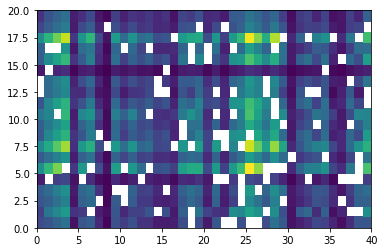
\includegraphics[width=.9\textwidth]{image/5_0.png}
    \caption{不完全なデータ行列$\bm A$}
    \end{minipage}
    \begin{minipage}{0.49\linewidth}
      \centering
      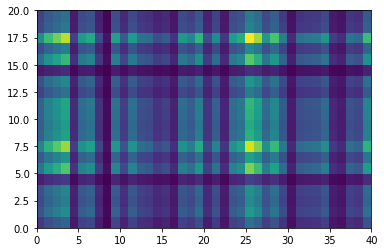
\includegraphics[width=.9\textwidth]{image/5_1.png}
    \caption{不完全なデータ行列$\bm A$から復元されたデータ$\bm Z$}
    \end{minipage}
  \end{figure}

  \item (Option: Additional 5 pts獲得可能) $\bm A$を復元するための代替アプローチとして非負行列因子分解を実装し、ハイパーパラメータを選択してパフォーマンスを比較する。ここで実装した2つの方法の長所と短所を説明してください。
\end{enumerate}
  
\end{document}
